\subsection{Zamiana kowariancji}
Zamiana kowariancji jest testem operującym na wielowymiarowych danych.
Test polega na rotacji współczynników macierzy kowariancji na podstawie,
której generowane są próbki
Wykres \ref{fig:CovValues} przedstawia przykładowe przebiegi wartości dla pierwszych 5 zmian
wraz z zaznaczonymi miejscami,
gdzie nastąpiła.
\begin{figure}[htbp]
  \centering
  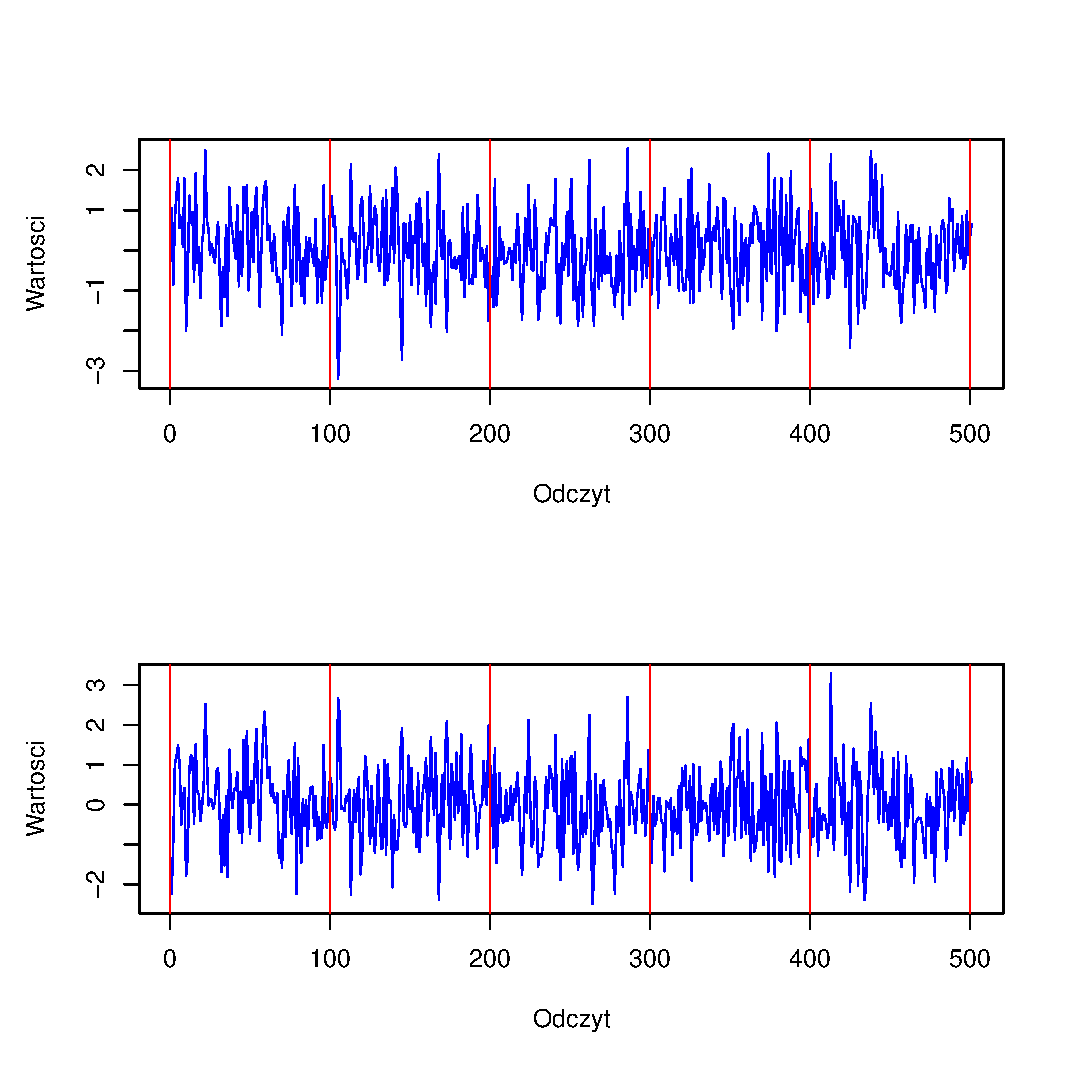
\includegraphics[width=0.8\textwidth]{img/ch-5-cov}
  \caption{Przykładowe wartości}
  \label{fig:CovValues}
\end{figure}
Dla poprawienia widoczności każdy z wymiarów została oznaczony na osobnych grafikach.
Na górnym rysunku przedstawiono pierwszy wymiar, na niższym drugi.

Na wykresie \ref{fig:CovValuesResTpr} przedstawiono współczynniki sukcesów otrzymanych podczas kolejnych prób.
Wśród pokazanych wyników nie ma $\mbox{ADWIN}_\mu$.
Algorytm ten oparty na teście wartości średnich z racji swojej konstrukcji nie był przygotowany do przyjmowania wielowymiarowych próbek.
Alternatywnie podczas testów sprawdzono jego skuteczność dla pojedynczych wymiarów.
Otrzymane wyniki okazały się nie wystarczające, ponieważ algorytm w ogóle albo prawie w cale nie wykrywał zmian.
Dlatego nie umieszczono go na narysowanych wykresach.
Pośród pozostałych widać wyraźną przewagę $\mbox{ADWIN}_d$ nad BAY.
Algorytm $\mbox{ADWIN}_d$ utrzymał swoją skuteczność na zbliżonym poziome co w przypadku testu na danych jednowymiarowych.
Niestety skuteczność BAY znacząco spadła.
\begin{figure}[htbp]
  \centering
  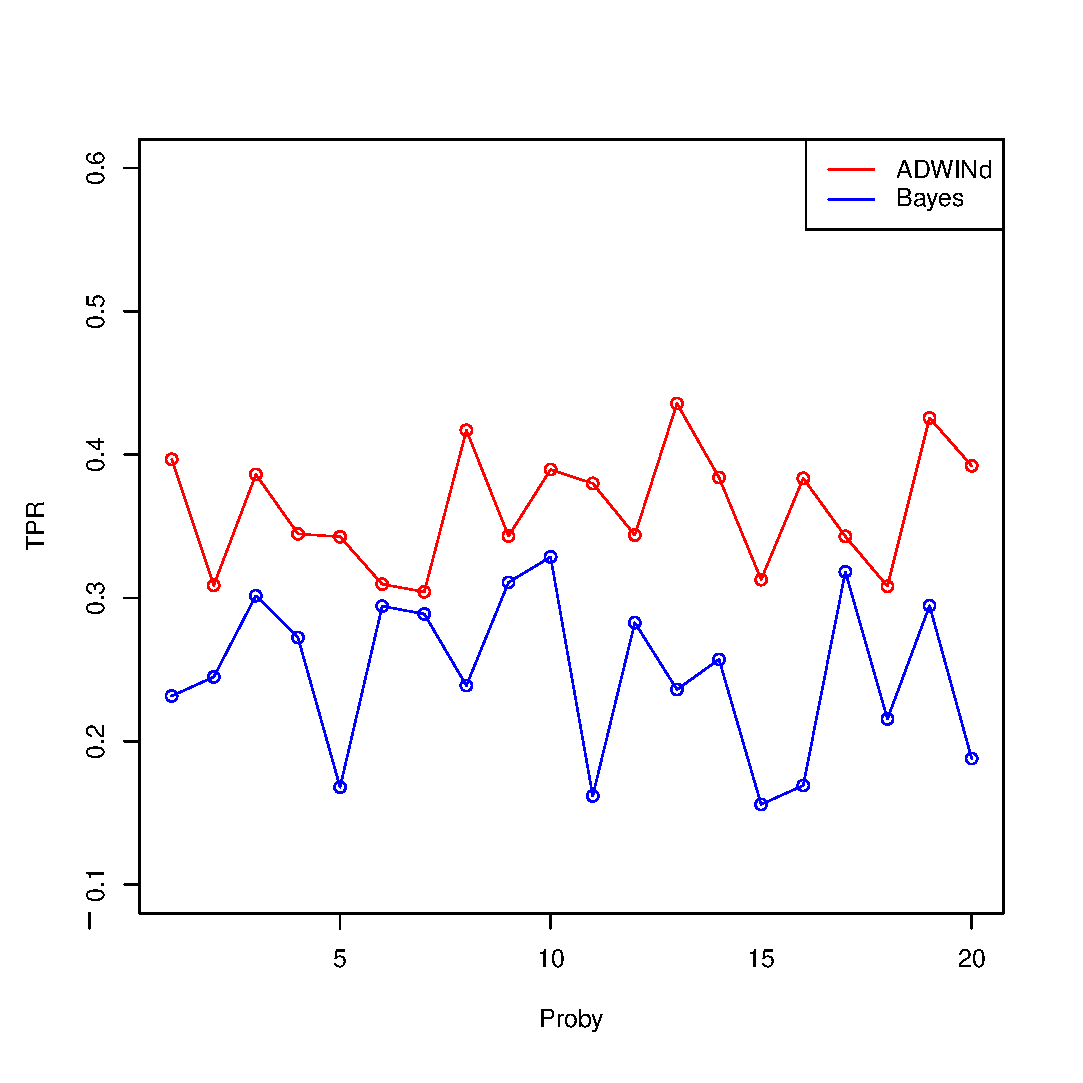
\includegraphics[width=0.6\textwidth]{img/ch-5-cov-res-tpr}
  \caption{Wyniki dla poszczególnych prób -- współczynnik sukcesów}
  \label{fig:CovValuesResTpr}
\end{figure}

Wykres \ref{fig:CovValuesResNpr} przedstawia informację o fałszywych alarmach.
Oś OX oznacza kolejne próby,
oś OY reprezentuje wartości współczynnika NPR.
W przypadku liczby fałszywych alarmów widać wyraźną poprawę analizowanych algorytmów w porównaniu do testu skaczącej średniej.
Jednak nie wynika ona z poprawy samych metod,
a ze specyfiki problemu.
Badane próbki zachowują stabilność,
a zachodzące zmiany są bardzo subtelne,
właściwie dla człowieka niezauważalne (rys. \ref{fig:CovValues}).
Powoduje to niską całościową liczbę wykrytych zmian przez algorytmy,
co naturalnie przekłada się na niską liczbę fałszywych alarmów.
\begin{figure}[htbp]
  \centering
  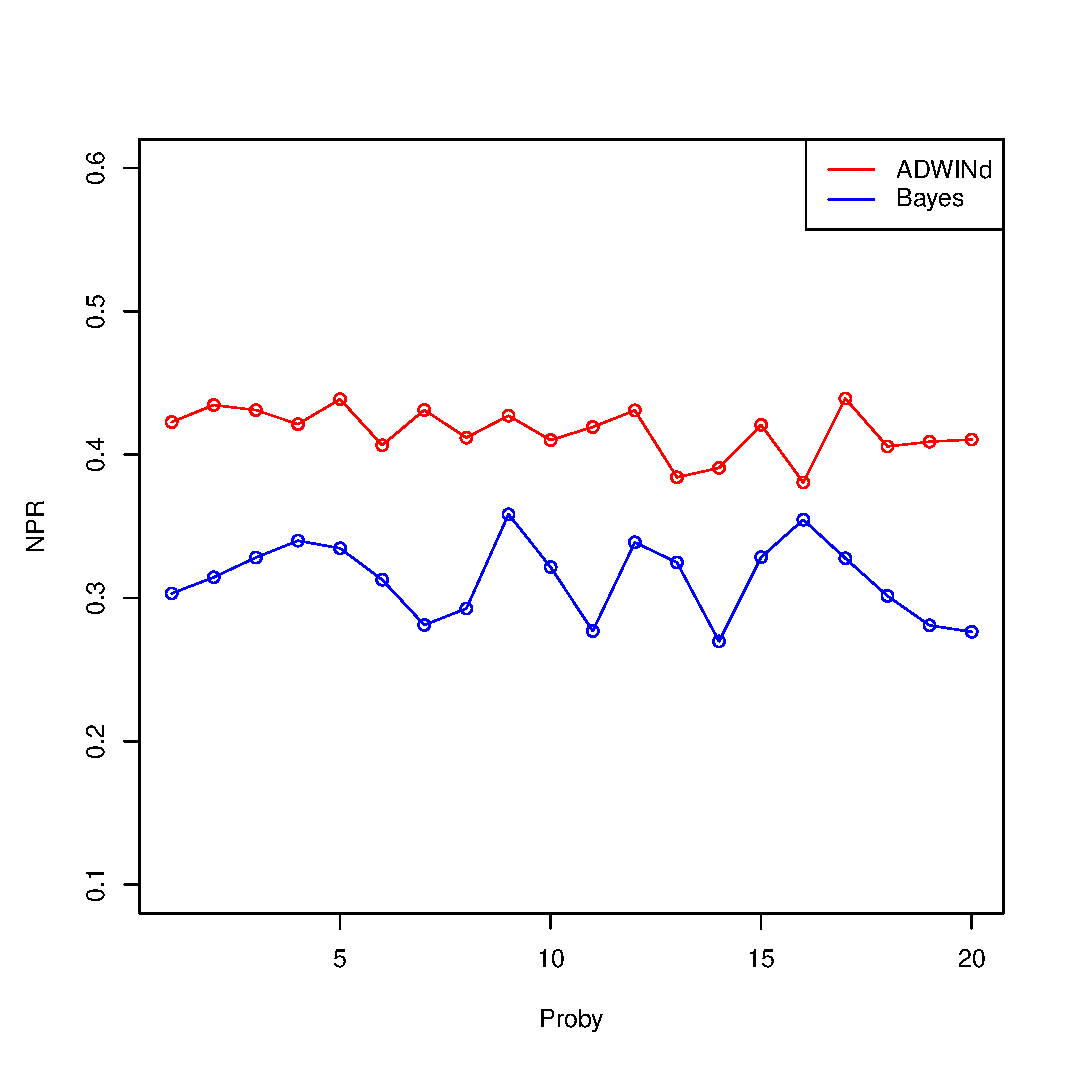
\includegraphics[width=0.6\textwidth]{img/ch-5-cov-res-npr}
  \caption{Wyniki dla poszczególnych prób -- fałszywe alarmy}
  \label{fig:CovValuesResNpr}
\end{figure}

W tabeli \ref{tab:CovResult} przedstawiono zbiorcze wyniki współczynników sukcesu i fałszywych alarmów.
\begin{table}[h]
  \label{tab:CovResult}
  \centering
  \begin{tabular}{l r r r r}
    & \multicolumn{2}{l}{TPR} & \multicolumn{2}{l}{NPR} \\
    \hline
    & \multicolumn{1}{l}{Średnia} & \multicolumn{1}{l}{Wariancja}& \multicolumn{1}{l}{Średnia} & \multicolumn{1}{l}{Wariancja} \\
    \hline
    BAY & 0,185 & $0,0728 \times 10^{-3}$ & 0,313 & $0,723 \times 10^{-3}$ \\
    $ADW_{d}$ & 0,363 & $1,623 \times 10^{-3}$ & 0,415 & $0,0291 \times 10^{-3}$ \\
  \end{tabular}
\end{table}
